\section{Model Evaluation and Selection}

\begin{frame}{Model Evaluation and Selection}
	\begin{itemize}
		\item \textbf{Evaluation metrics:}
		      \begin{itemize}
			      \item How can we measure accuracy?
			      \item Other metrics to consider?
		      \end{itemize}
		\item \textbf{Use {\color{airforceblue}test} set of class-labeled tuples instead of training set when assessing accuracy.}
		\item \textbf{Methods for estimating a classifier's accuracy:}
		      \begin{itemize}
			      \item Holdout method, random subsampling.
			      \item Cross-validation.
			      \item Bootstrap.
		      \end{itemize}
		\item \textbf{Comparing classifiers:}
		      \begin{itemize}
			      \item Confidence intervals.
			      \item Cost-benefit analysis and ROC curves.
		      \end{itemize}
	\end{itemize}
\end{frame}

\begin{frame}{Model Evaluation and Selection (II)}
	\begin{itemize}
		\item \textbf{Confusion Matrix:}\\[0.2cm]
		      \begin{tabular}{|c|c|c|}
			      \hline
			      Actual class/predicted class: & $C_1$                         & $\neg C_1$                    \\\hline
			      $C_1$                         & \textbf{True positives (TP)}  & \textbf{False negatives (FN)} \\\hline
			      $\neg C_1$                    & \textbf{False positives (FP)} & \textbf{True negatives (TN)}  \\\hline
		      \end{tabular}
		\item \textbf{Example:}\\[0.2cm]
		      \begin{tabular}{|c|c|c|c|}
			      \hline
			      Actual class/predicted class: & buys\_computer = yes & buys\_computer = no & Total \\\hline
			      buys\_computer = yes          & \textbf{6954}        & \textbf{46}         & 7000  \\\hline
			      buys\_computer = no           & \textbf{412}         & \textbf{2588}       & 3000  \\\hline
			      Total                         & 7366                 & 2634                & 10000 \\\hline
		      \end{tabular}
		\item Given $M$ classes, an entry $C^{(m)}_{ij}$ in an $M \times M$ confusion matrix indicates \# of tuples in class $i$ that were labeled by the classifier as class $j$.
		\item May have extra rows/columns to provide totals.
	\end{itemize}
\end{frame}

\begin{frame}{Classifier-evaluation Metrics: Accuracy, Error Rate, Sensitivity and Specificity}
	\begin{columns}
		\begin{column}{0.5\textwidth}
			\centering
			\begin{tabular}{|c|c|c|c|}
				\hline
				A/P      & C           & $\neg$ C    &              \\\hline
				C        & \textbf{TP} & \textbf{FN} & \textbf{P}   \\\hline
				$\neg$ C & \textbf{FP} & \textbf{TN} & \textbf{N}   \\\hline
				         & \textbf{P}' & \textbf{N}' & \textbf{All} \\\hline
			\end{tabular}
			\begin{itemize}
				\item \textbf{Classifier accuracy, or recognition rate:}
				      \begin{itemize}
					      \item Percentage of test set tuples that are correctly classified.
					      \item $\text{Accuracy} = \frac{\text{TP} + \text{TN}}{\text{All}}.$
					      \item \textbf{Error rate:}
					            \begin{itemize}
						            \item $1-\text{accuracy}$, or
						            \item $\text{Error rate} = \frac{\text{FP}+\text{FN}}{\text{All}}.$
					            \end{itemize}
				      \end{itemize}
			\end{itemize}
		\end{column}
		\begin{column}{0.5\textwidth}
			\begin{itemize}
				\item \textbf{Class-imbalance problem:}
				      \begin{itemize}
					      \item One class may be rare e.g., fraud, or HIV-positive.
					      \item Significant majority of the negative class and minority of the positive class
					      \item \textbf{Sensitivity:} True-positive recognition rate. $\text{Sensitivity} = \frac{TP}{P}$.
					      \item \textbf{Specificity:} False-negative recognition rate. $\text{Specificity} = \frac{TN}{N}$.
				      \end{itemize}
			\end{itemize}
		\end{column}
	\end{columns}
\end{frame}

\begin{frame}{Classifier-evaluation Metrics: Precision, Recall, and F-measures}
	\begin{itemize}
		\item \textbf{Precision:}
		      \begin{itemize}
			      \item Exactness -- the $\%$ of tuples that are actually positive \\
			            in those that the classifier labeled as positive: $\frac{\text{TP}}{\text{TP} + \text{FP}}$.
		      \end{itemize}
		\item \textbf{Recall:}
		      \begin{itemize}
			      \item Completeness -- the $\%$ of tuples that the classifier labeled \\
			            as positive in all positive tuples: $\frac{\text{TP}}{\text{TP} + \text{FN}}$.
			      \item Perfect score is $1.0$.
		      \end{itemize}
		\item \textbf{Inverse relationship between precision and recall.}% TODO: bezeichnung inverse evtl verwirrend
		\item \textbf{F-measure ($F_1$ or $F$-score):}
		      \begin{itemize}
			      \item Gives equal weight to precision and recall: $F = \frac{2\cdot\text{precision}\cdot \text{recall}}{\text{precision} + \text{recall}}$.
		      \end{itemize}
		\item \textbf{$F_\beta$ weighted measure of precision and recall:}
		      \begin{itemize}
			      \item Assigns $\beta$ times as much weight to recall as to precision: $F_\beta = \frac{(1+\beta^2) \cdot \text{precision} \cdot \text{recall}}{\beta^2 \cdot \text{precision} + \text{recall}}$.
		      \end{itemize}
	\end{itemize} % TODO: (1+beta)^2 oder (1+beta^2) - wie ist F-beta measure definiert
\end{frame}

\begin{frame}{Classifier-evaluation Metrics: Precision, Recall, and F-measures (II)}
	\centering
	\begin{tabular}{|c|c|c|c|c|}
		\hline
		Actual class/predicted class & cancer = yes & cancer = no   & Total & Recognition ($\%$)  \\\hline
		cancer = yes                 & \textbf{90}  & \textbf{210}  & 300   & 30.00 (sensitivity) \\\hline
		cancer = no                  & \textbf{140} & \textbf{9560} & 9700  & 98.56 (specificity) \\\hline
		Total                        & 230          & 9770          & 10000 & 96.40 (accuracy)    \\\hline
	\end{tabular}\\[0.2cm]
	\begin{itemize}
		\item Precision $= \frac{90}{230} = 39.13 \%$.
		\item Recall $=\frac{90}{300} = 30.00 \%$.
		\item $F_1$-measure = $\frac{2 \cdot 0.3913 \cdot 0.3}{0.3913 + 0.3} = 33.96 \%$.
	\end{itemize}
\end{frame}

\begin{frame}{Classifier-evaluation Metrics: Holdout \& Cross-validation Methods}
	\begin{itemize}
		\item \textbf{Holdout method.}
		      \begin{itemize}
			      \item Given data is randomly partitioned into two independent sets:
			            \begin{itemize}
				            \item \textbf{\color{airforceblue}Training set} (E.g., $2/3$) for model construction.
				            \item \textbf{\color{airforceblue}Test set} (E.g., $1/3$) for accuracy estimation.
			            \end{itemize}
			      \item Random sampling: a variation of holdout.
			            \begin{itemize}
				            \item Repeat holdout $k$ times, accuracy = avg. of the accuracies obtained.
			            \end{itemize}
		      \end{itemize}
		\item \textbf{{\color{airforceblue}Cross-validation} ($k$-fold, where $k = 10$ is most popular).}
		      \begin{itemize}
			      \item Randomly partition the data into $k$ mutually exclusive subsets, each approximately equal size.
			      \item At $i$-th iteration, use $D_i$ as test set and the others as training set.
			      \item Leave-one-out: $k$ folds, where $k = \#$ of tuples; for small-sized data.
			      \item Stratified cross-validation: Folds are stratified so that class distribution in each fold is approx. the same as that in the initial data.
		      \end{itemize}
	\end{itemize}
\end{frame}

\begin{frame}{Evaluating Classifier Accuracy: Bootstrap}
	\begin{itemize}
		\item \textbf{Bootstrap.}
		      \begin{itemize}
			      \item Works well with small data sets.
			      \item Samples the given training tuples uniformly with replacement.
			            \begin{itemize}
				            \item I.e. each time a tuple is selected, it is equally likely \\
				                  to be selected again and re-added to the training set.
			            \end{itemize}
		      \end{itemize}
		\item \textbf{Several bootstrap methods, and a common one is $.632$ bootstrap.}
		      \begin{itemize}
			      \item Data set with $d$ tuples sampled d times, with replacement, \\
			            resulting in a training set of $d$ samples.
			      \item The data tuples that did not make it into the training set end up forming the test set.
			            \begin{itemize}
				            \item About $63.2\%$ of the original data end up in the bootstrap, and the remaining $36.8\%$ form the test set (since $(1-\frac{1}{d})^d \approx e^{-1} = 0.368)$.
			            \end{itemize}
			      \item Repeat the sampling procedure $k$ times; overall accuracy of the model:
			            \begin{align}
				            \text{Acc}(M) = \frac{1}{k} \sum_{i=1}^{k} 0.632 \cdot \text{Acc}(M_i)_{\text{test\_set}} + 0.368 \cdot \text{Acc}(M_i)_{\text{train\_set}}.
			            \end{align}
		      \end{itemize}
	\end{itemize}
\end{frame}

\begin{frame}{Evaluating Classifier Accuracy: Bootstrap (II)}
	\begin{itemize}
		\item \textbf{Suppose we have $2$ classifiers, $M_1$ and $M_2$, which one is better?}
		\item \textbf{Use $10$-fold cross-validation to obtain $\overline{\text{err}}(M_1)$ and $\overline{\text{err}}(M_2)$.}
		      \begin{itemize}
			      \item Recall: error rate is $1-\text{accuracy}(M)$.
		      \end{itemize}
		\item \textbf{Mean error rates:}
		      \begin{itemize}
			      \item Just estimates of error on the true population of future data cases.
		      \end{itemize}
		\item \textbf{What if the difference between the $2$ error rates is just attributed to chance?}
		      \begin{itemize}
			      \item Use a test of statistical significance.
			      \item Obtain confidence limits for our error estimates.
		      \end{itemize}
	\end{itemize}
\end{frame}

\begin{frame}{Evaluating Classifier Accuracy: Null Hypothesis}
	\begin{itemize}
		\item \textbf{Perform $10$-fold cross-validation.}
		      \begin{itemize}
			      \item $10$ times.
		      \end{itemize}
		\item \textbf{Assume samples follow a $t$-distribution with $k-1$ degrees of freedom.}
		      \begin{itemize}
			      \item Here, $k = 10$.
		      \end{itemize}
		\item \textbf{Use $t$-test}
		      \begin{itemize}
			      \item Student's $t$-test.
		      \end{itemize}
		\item \textbf{Null hypothesis:}
		      \begin{itemize}
			      \item $M_1$ and $M_2$ are the same.
		      \end{itemize}
		\item \textbf{If we can reject the null hypothesis, then}
		      \begin{itemize}
			      \item Conclude that difference between $M_1$ and $M_2$ is statistically significant.
			      \item Obtain confidence limits for our error estimates.
		      \end{itemize}
	\end{itemize}
\end{frame}

\begin{frame}{Estimating Confidence Intervals: $t$-Test}
	\begin{itemize}
		\item \textbf{If only one test set available: pairwise comparison:}
		      \begin{itemize}
			      \item For $i$-th round of $10$-fold cross-validation, the same cross partitioning is used to obtain $\text{err}(M_1)_i$ and $\text{err}(M_2)_i$.
			      \item Average over $10$ rounds to get $\overline{\text{err}}(M_1)$ and $\overline{\text{err}}(M_2)$.
			      \item $t$-test computes $t$-statistic with $k-1$ degrees of freedom:
			            \begin{align}
				            \resizebox{3cm}{!}{%
					            $t = \frac{\overline{\text{err}}(M_1)- \overline{\text{err}}(M_2)}{\sqrt{\frac{\text{var}(M_1-M_2)}{k}}},$}
			            \end{align}
			      \item where
			            \begin{align}
				            \resizebox{10cm}{!}{%
					            $\text{var}(M_1-M_2) = \frac{1}{k} \sum_{i=1}^{k} \left[ \text{err}(M_1)_i - \text{err}(M_2)_i - (\overline{\text{err}}(M_1) - \overline{\text{err}}(M_2))\right]^2.$}
			            \end{align}
		      \end{itemize}
		\item \textbf{If two test sets available: use nonpaired $t$-test:}
		      \begin{align}
			      \resizebox{5cm}{!}{%
				      $\text{var}(M_1-M_2) = \sqrt{\frac{\text{var}(M_1)}{k_1} + \frac{\text{var}(M_2)}{k_2}},$}
		      \end{align}
		      where $k_1$ \& $k_2$ are $\#$ of cross-validation samples used for $M_1$ \& $M_2$, respectively.
	\end{itemize}
\end{frame}

\begin{frame}{Estimating Confidence Intervals: Table for $t$-Distribution}
	\begin{columns}
		\begin{column}{0.5\textwidth}
			\vspace{-6cm}
			\centering
			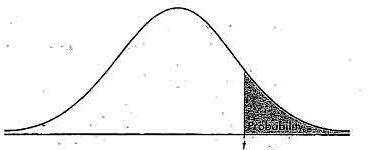
\includegraphics[width=0.8\textwidth]{img/ttest1.jpeg}
			\begin{itemize}
				\item Symmetrical.
				\item \textbf{\color{airforceblue}Significance level}:
				      \begin{itemize}
					      \item E.g., $\text{sig} = 0.05$ or $5\%$ means $M_1$ \& $M_2$ are significantly different for $95\%$ of population.
				      \end{itemize}
				\item Confidence limit: $z = \frac{\text{sig}}{2}$.
			\end{itemize}
		\end{column}
		\begin{column}{0.5\textwidth}
			\centering
			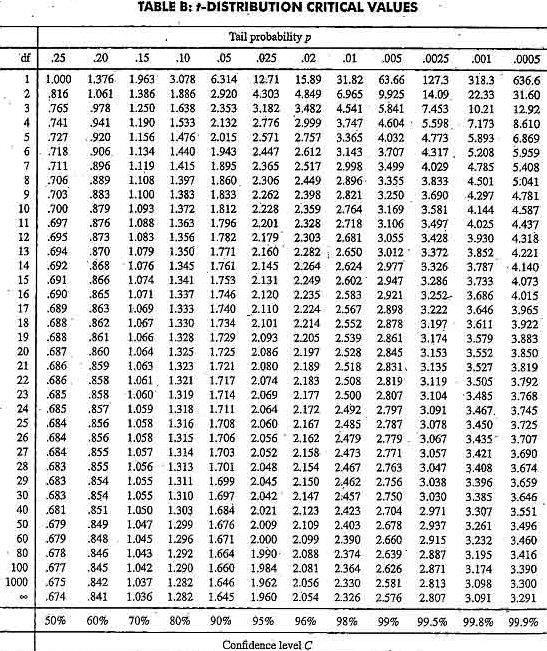
\includegraphics[width=0.7\textwidth]{img/ttest2.jpeg}
		\end{column}
	\end{columns}
\end{frame}

\begin{frame}{Estimating Confidence Intervals: Statistical Significance}
	\textbf{Are $M_1$ and $M_2$ {\color{airforceblue} significantly different}?}
	\begin{itemize}
		\item Compute $t$. Select significance level (E.g., sig = $5 \%$).
		\item Consult table for $t$-distribution:
		      \begin{itemize}
			      \item $t$-distribution is symmetrical:
			            \begin{itemize}
				            \item Typically upper $\%$ points of distribution shown.
			            \end{itemize}
			      \item Find critical value $c$ corresponding to $k-1$ degrees of freedom (here, $9$)
			      \item and for confidence limit $z = \frac{\text{sig}}{2}$ (here, $0.025$).
			      \item $\implies$ Here, critical value $c = 2.262$
		      \end{itemize}
		\item If $t > c$ or $t < -c$, then $t$ value lies in rejection region:
		      \begin{itemize}
			      \item \textbf{Reject null hypothesis} that mean error rates of $M_1$ and $M_2$ are equal.
			      \item Conclude: \textbf{statistically significant difference} between $M_1$ and $M_2$.
		      \end{itemize}
		\item Otherwise, conclude that any difference is chance.
	\end{itemize}

\end{frame}

\begin{frame}{Model Selection: ROC-Curves}
	\begin{columns}
		\begin{column}{0.6\textwidth}
			\begin{itemize}
				\item \textbf{ROC (Receiver Operating Characteristics) curves:}
				      \begin{itemize}
					      \item For visual comparison of classification models.
					      \item Originated from signal-detection theory.
					      \item Shows the trade-off between the true-positive rate and the false-positive rate.
				      \end{itemize}
				\item \textbf{The area under the ROC curve is a {\color{airforceblue}measure of the accuracy} of the model.}
				\item \textbf{{\color{airforceblue}Rank the test tuples} in decreasing order:}
				      \begin{itemize}
					      \item The one that is most likely to belong to the positive class appears at the top of the list.
				      \end{itemize}
				\item \textbf{The closer to the diagonal line (i.e. the closer the area is to $0.5$), the less accurate is the model.}
			\end{itemize}
		\end{column}
		\begin{column}{0.4\textwidth}
			\vspace{-1cm}
			\centering
			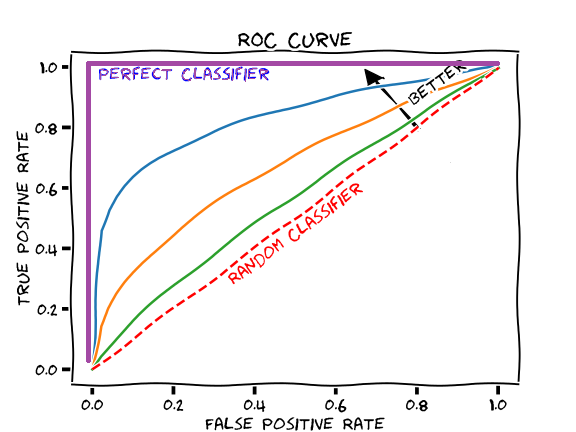
\includegraphics[width=\textwidth]{img/roc-curve.png}
			\begin{itemize}
				\item Vertical axis represents TP.
				\item Horizontal axis repr. the FP.
				\item The plot also shows a diagonal line.
				\item A model with perfect accuracy will have an area of $1.0$.
			\end{itemize}
		\end{column}
	\end{columns}
\end{frame}

\begin{frame}{Issues after Model Selection}
	\begin{itemize}
		\item \textbf{Accuracy.}
		      \begin{itemize}
			      \item Classifier accuracy: predicting class label.
		      \end{itemize}
		\item \textbf{Speed.}
		      \begin{itemize}
			      \item Time to construct the model (training time).
			      \item Time to use the model (classification/prediction time).
		      \end{itemize}
		\item \textbf{Robustness.}
		      \begin{itemize}
			      \item Handling noise and missing values.
		      \end{itemize}
		\item \textbf{Scalability.}
		      \begin{itemize}
			      \item Efficiency in disk-resident databases.
		      \end{itemize}
		\item \textbf{Interpretability.}
		      \begin{itemize}
			      \item Understanding and insight provided by the model.
		      \end{itemize}
		\item \textbf{Other measures.}
		      \begin{itemize}
			      \item E.g., goodness of rules, such as decision-tree size or compactness of classification rules.
		      \end{itemize}
	\end{itemize}
\end{frame}
